
This study aims at exposing, with the help of energy flow 
networks~\cite{Komiske:2018cqr}, new features of jets induced by higher-order
corrections to parton showers, using the \textsc{Dire} parton shower~\cite{Hoche:2015sya}
as a test case.

Parton shower programs are an an important aspect
of LHC phenomenology, since they imprint perturbative all-order effects onto the
jet structure produced by Event Generators. As such, they serve two primary
purposes: $1)$ the distribution of low-multiplicity
(hard-scattering) states over states of arbitrarily high multiplicity, as well
as $2)$ generating the effect of resummation for observable depending only on 
low-multiplicity configurations. These two goals often lead to conflicting
requirements, as e.g.\ choices to improve
$2)$ often limit the potential to improve $1)$ -- and vice versa. Luckily,
these conflicts are not directly apparent at lowest (i.e.\ leading) order. This
has resulted in parton showers being ``stuck" at leading-order 
(leading-logarithmic) accuracy in their description of emission and 
no-emission rates. With increased demand for more precise event generation, 
improved parton showers will become necessary at the LHC and beyond. For 
example, the use of NLO PDFs (as e.g.\ mandated in NLO+PS
matching) in the parton shower in principle requires parton showers beyond
lowest order.

One way to improve the all-order behavior of the parton shower (point $2)$ 
above while preserving a systematically improvable state distribution (point $1)$ 
above is to consistently include higher-order and higher-multiplicity 
splitting functions in the parton 
shower~\cite{Li:2016yez, Hoche:2017iem,Dulat:2018vuy}. Some of the 
necessary ingredients at NLO are shown in 
Fig.~\ref{fig:jets:np:triplecollineardiagrams}. 
At leading order, these configurations are approximated through the iterated 
application of leading-order splittings. This approximation however may
yield an incorrect distribution\footnote{\dots e.g.\ if the polarisation of 
the intermediate gluon in 
Figs.~\ref{fig:jets:np:triplecollineardiagrams1}-\ref{fig:jets:np:triplecollineardiagrams4},
\ref{fig:jets:np:triplecollineardiagrams7}-\ref{fig:jets:np:triplecollineardiagrams8}
is omitted, leading to an incorrect modulation of azimuthal angles,
or by disregarding the interference between
$C_F$-type and $C_A$-type color structures from 
Figs.~\ref{fig:jets:np:triplecollineardiagrams7}-\ref{fig:jets:np:triplecollineardiagrams8}.}
or may be limited to phase-space regions constrained by successive 
ordering requirements\footnote{\dots easily leading to the 
incorrect overall phase space volume, and thus failing to recover known anomalous
dimensions upon integration.}.
The correct final result is obtained by including the 
complete configurations in Fig.~\ref{fig:jets:np:triplecollineardiagrams}
as new rates in the parton shower, and subtracting from these new rates
the leading-order result. This subtraction will, given a suitable definition
of the leading-order shower, act to ensure local finiteness of the new, 
subtracted, rates. We will call these subtracted rates ``NLO corrections".

In~\cite{Hoche:2017iem}, triple-collinear corrections from diagrams
similar to~\ref{fig:jets:np:triplecollineardiagrams2} were considered, with
the difference that instead of the primary parton (indicated with a double 
line), one of the quarks in the loop was considered as ``hard". Such
configurations give rise, upon integration, to the flavor-changing 
DGLAP kernels $P_{qq'}$ and $P_{q\bar q}$. We will call this 
``triple-collinear" correction. The calculation of these corrections has
helped define a method to use the overlap with lowest order to construct 
locally finite splitting rates at NLO. Numerically however, this correction is 
expected to be small to modest.
The soft limits of all the diagrams in Fig.~\ref{fig:jets:np:triplecollineardiagrams}
was considered in~\cite{Dulat:2018vuy}, which also included all necessary 
virtual corrections obtained by moving the cuts in the individual diagrams in 
all possible ways. We will call this ``double-soft" correction\footnote{
It should be noted that there is overlap between the
triple-collinear and double-soft limits. A complete differential calculation 
that consistently (i.e.\ without overlap) includes all components has yet
to be produced. Thus, we assess the potential to find observables
that discriminate between leading-order and next-to-leading order
results separately, for triple-collinear, and for double-soft corrections.}. 
The numerical effect of these double-soft corrections is expected to be appreciable.

In this study, we use the implementation of the triple-collinear and 
double-soft corrections in \textsc{Dire} to produce NLO pseudo-data, with the aim
of highlighting the characteristic new features of either correction.

Events are treated as sets of particles, with each particle $p_i$ specified by its momentum $\vec p_i^\mu$, mass, and particle-type.
%
The events are rotated to a consistent orientation by vertically aligning the second moment of the energy flow~\cite{Komiske:2019asc}.
%
This is accomplished by diagonalizing the spatial component of $\mathcal I^{\mu\nu} = \sum_{i=1}^M E_i v_i^\mu v_i^\nu$, where $v_i^\mu = p_i^\mu/E_i$ is the particle velocity.
As a machine learning architecture to process the entire events in their natural representation as sets of particles, we use Particle Flow Networks (PFNs)~\cite{Komiske:2018cqr} (see also Ref.~\cite{DBLP:conf/nips/ZaheerKRPSS17}).
%
Intuitively, PFNs learn a collection of additive observables which are processed by a fully-connected network.
%
A PFN acts on an event with $M$ particles $p_i$ as $\text{PFN}(\{p_i\}_{i=1}^M) = F\left(\sum_{i=1}^M \Phi(p_i)\right)$, where $F$ and $\Phi$ are parameterized by dense networks.
%
The network sizes of $F$ and $\Phi$ are identical to those in Ref.~\cite{Komiske:2018cqr}, with a latent space dimension of 256.
%
The train, validation, and test set sizes were 175k, 10k, and 15k, respectively.
%
The PFN classifiers were trained for 25 epochs with a batch size of 500.

Receiver operating characteristic (ROC) curves from the machine learning classifiers are presented in Fig.~\ref{fig:jets:np:triplecollinearNN}.  These curves show the performance of a classifier designed to distinguish the default simulation from one that includes either the triple collinear splitting function or the double soft splitting function.  A neural network is compared with a simple classifier that only uses the jet constituent multiplicity.  We find that the effect triple-collinear corrections (which integrate to
the DGLAP kernels $P_{qq'}$ and $P_{q\bar q}$) is difficult to pinpoint. 
It is somewhat surprising that the impact is almost vanishing.  Furthermore, we find that double-soft corrections have sizable impact, and can
easily be filtered out of the data. This is expected, since the theoretical
description of soft gluons changes significantly.  It is currently unclear what features the neural network is using to distinguish the default simulation from the one that includes the double soft splitting function.  Figure~\ref{fig:jets:np:triplecollinearNN} indicates that the network is using more than just the jet constituent multiplicity.  Future studies will be required to identify a suitable observable to measure (perhaps the neural network itself).  

\begin{figure}[h!]
\subfigure[]{
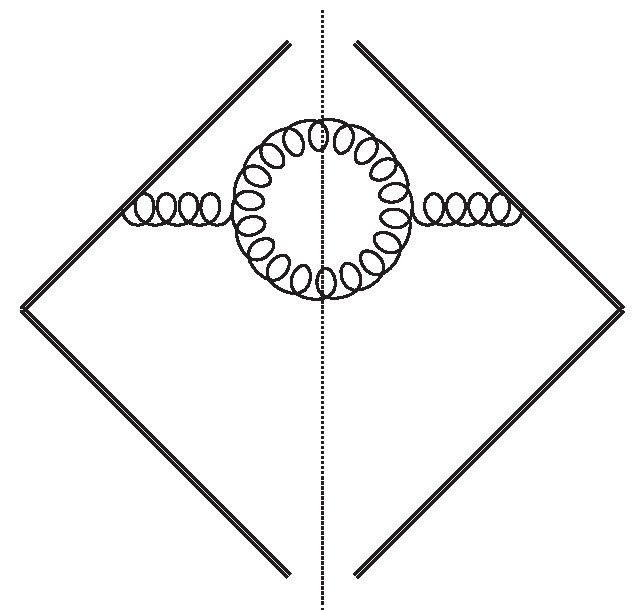
\includegraphics[width=0.23\textwidth]{figs/nlo_real_vpcg.pdf}
\label{fig:jets:np:triplecollineardiagrams1}
}
\subfigure[]{
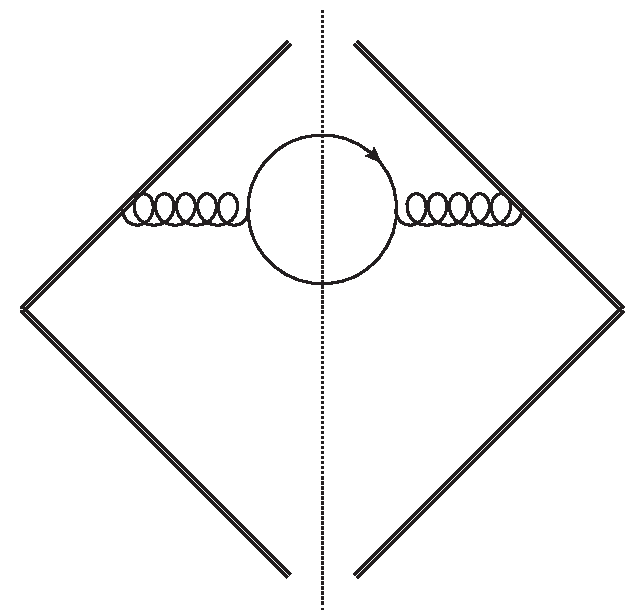
\includegraphics[width=0.23\textwidth]{figs/nlo_real_vpcq.pdf}
\label{fig:jets:np:triplecollineardiagrams2}
}
\subfigure[]{
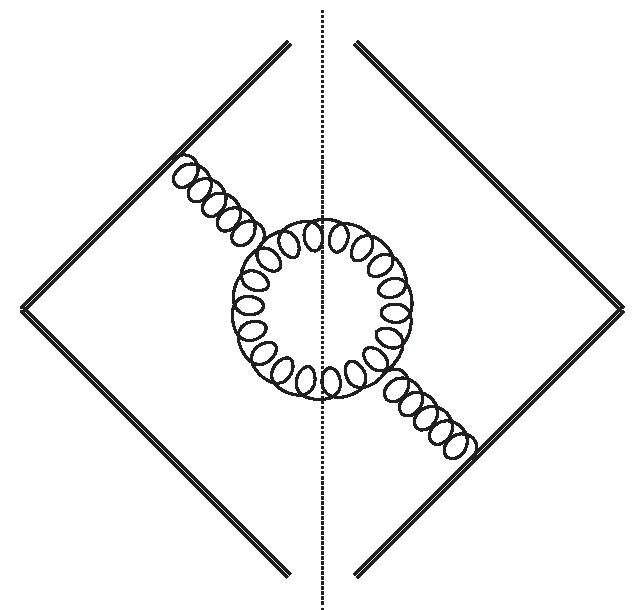
\includegraphics[width=0.23\textwidth]{figs/nlo_real_vpsg.pdf}
\label{fig:jets:np:triplecollineardiagrams3}
}
\subfigure[]{
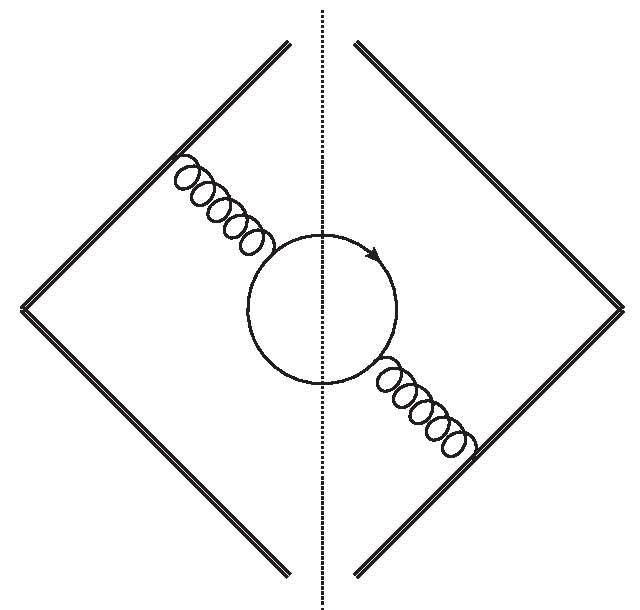
\includegraphics[width=0.23\textwidth]{figs/nlo_real_vpsq.pdf}
\label{fig:jets:np:triplecollineardiagrams4}
}
\\
\subfigure[]{
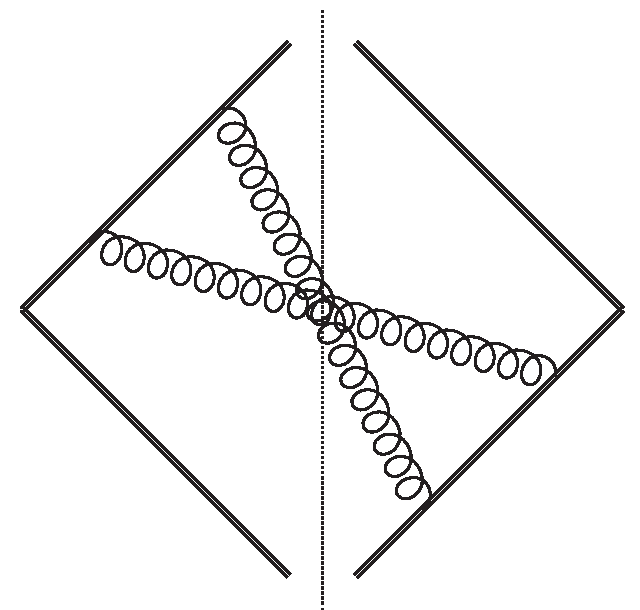
\includegraphics[width=0.23\textwidth]{figs/nlo_real_box1.pdf}
\label{fig:jets:np:triplecollineardiagrams5}
}
\subfigure[]{
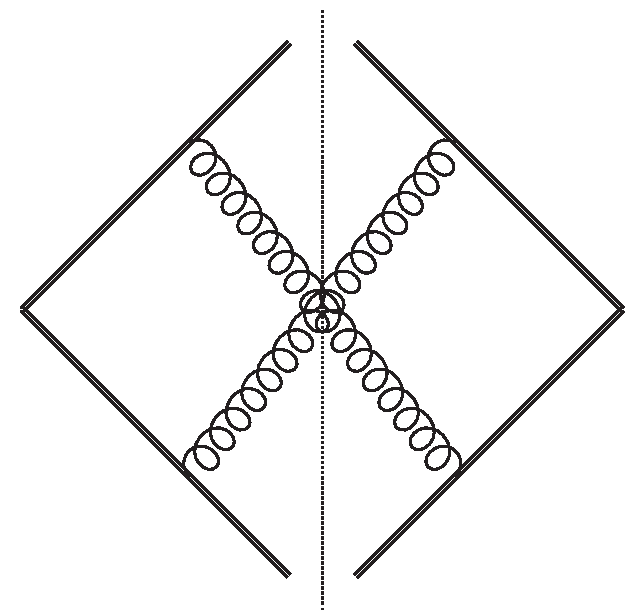
\includegraphics[width=0.23\textwidth]{figs/nlo_real_box2.pdf}
\label{fig:jets:np:triplecollineardiagrams6}
}
\subfigure[]{
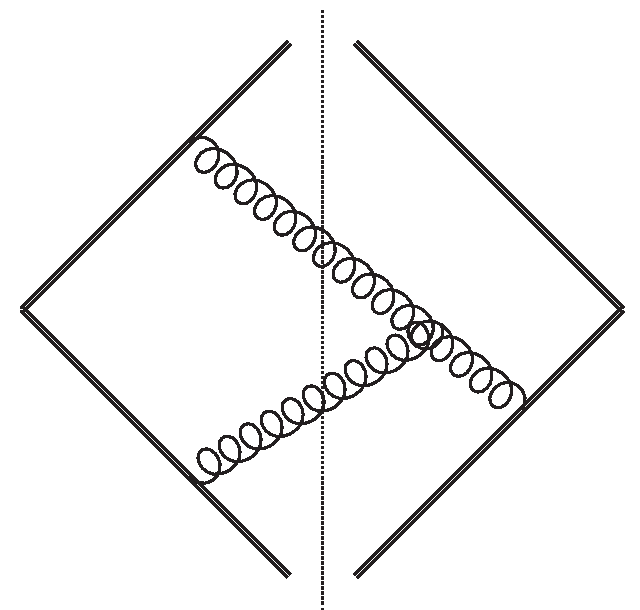
\includegraphics[width=0.23\textwidth]{figs/nlo_real_tgc1.pdf}
\label{fig:jets:np:triplecollineardiagrams7}
}
\subfigure[]{
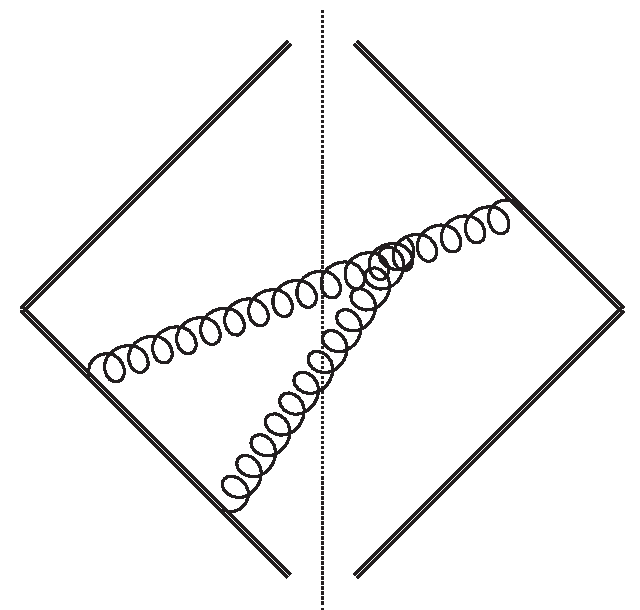
\includegraphics[width=0.23\textwidth]{figs/nlo_real_tgc2.pdf}
\label{fig:jets:np:triplecollineardiagrams8}
}
\caption{Examples of parton shower configurations required to go beyond leading order.}
\label{fig:jets:np:triplecollineardiagrams}
\end{figure}

\begin{figure}[h!]
\centering
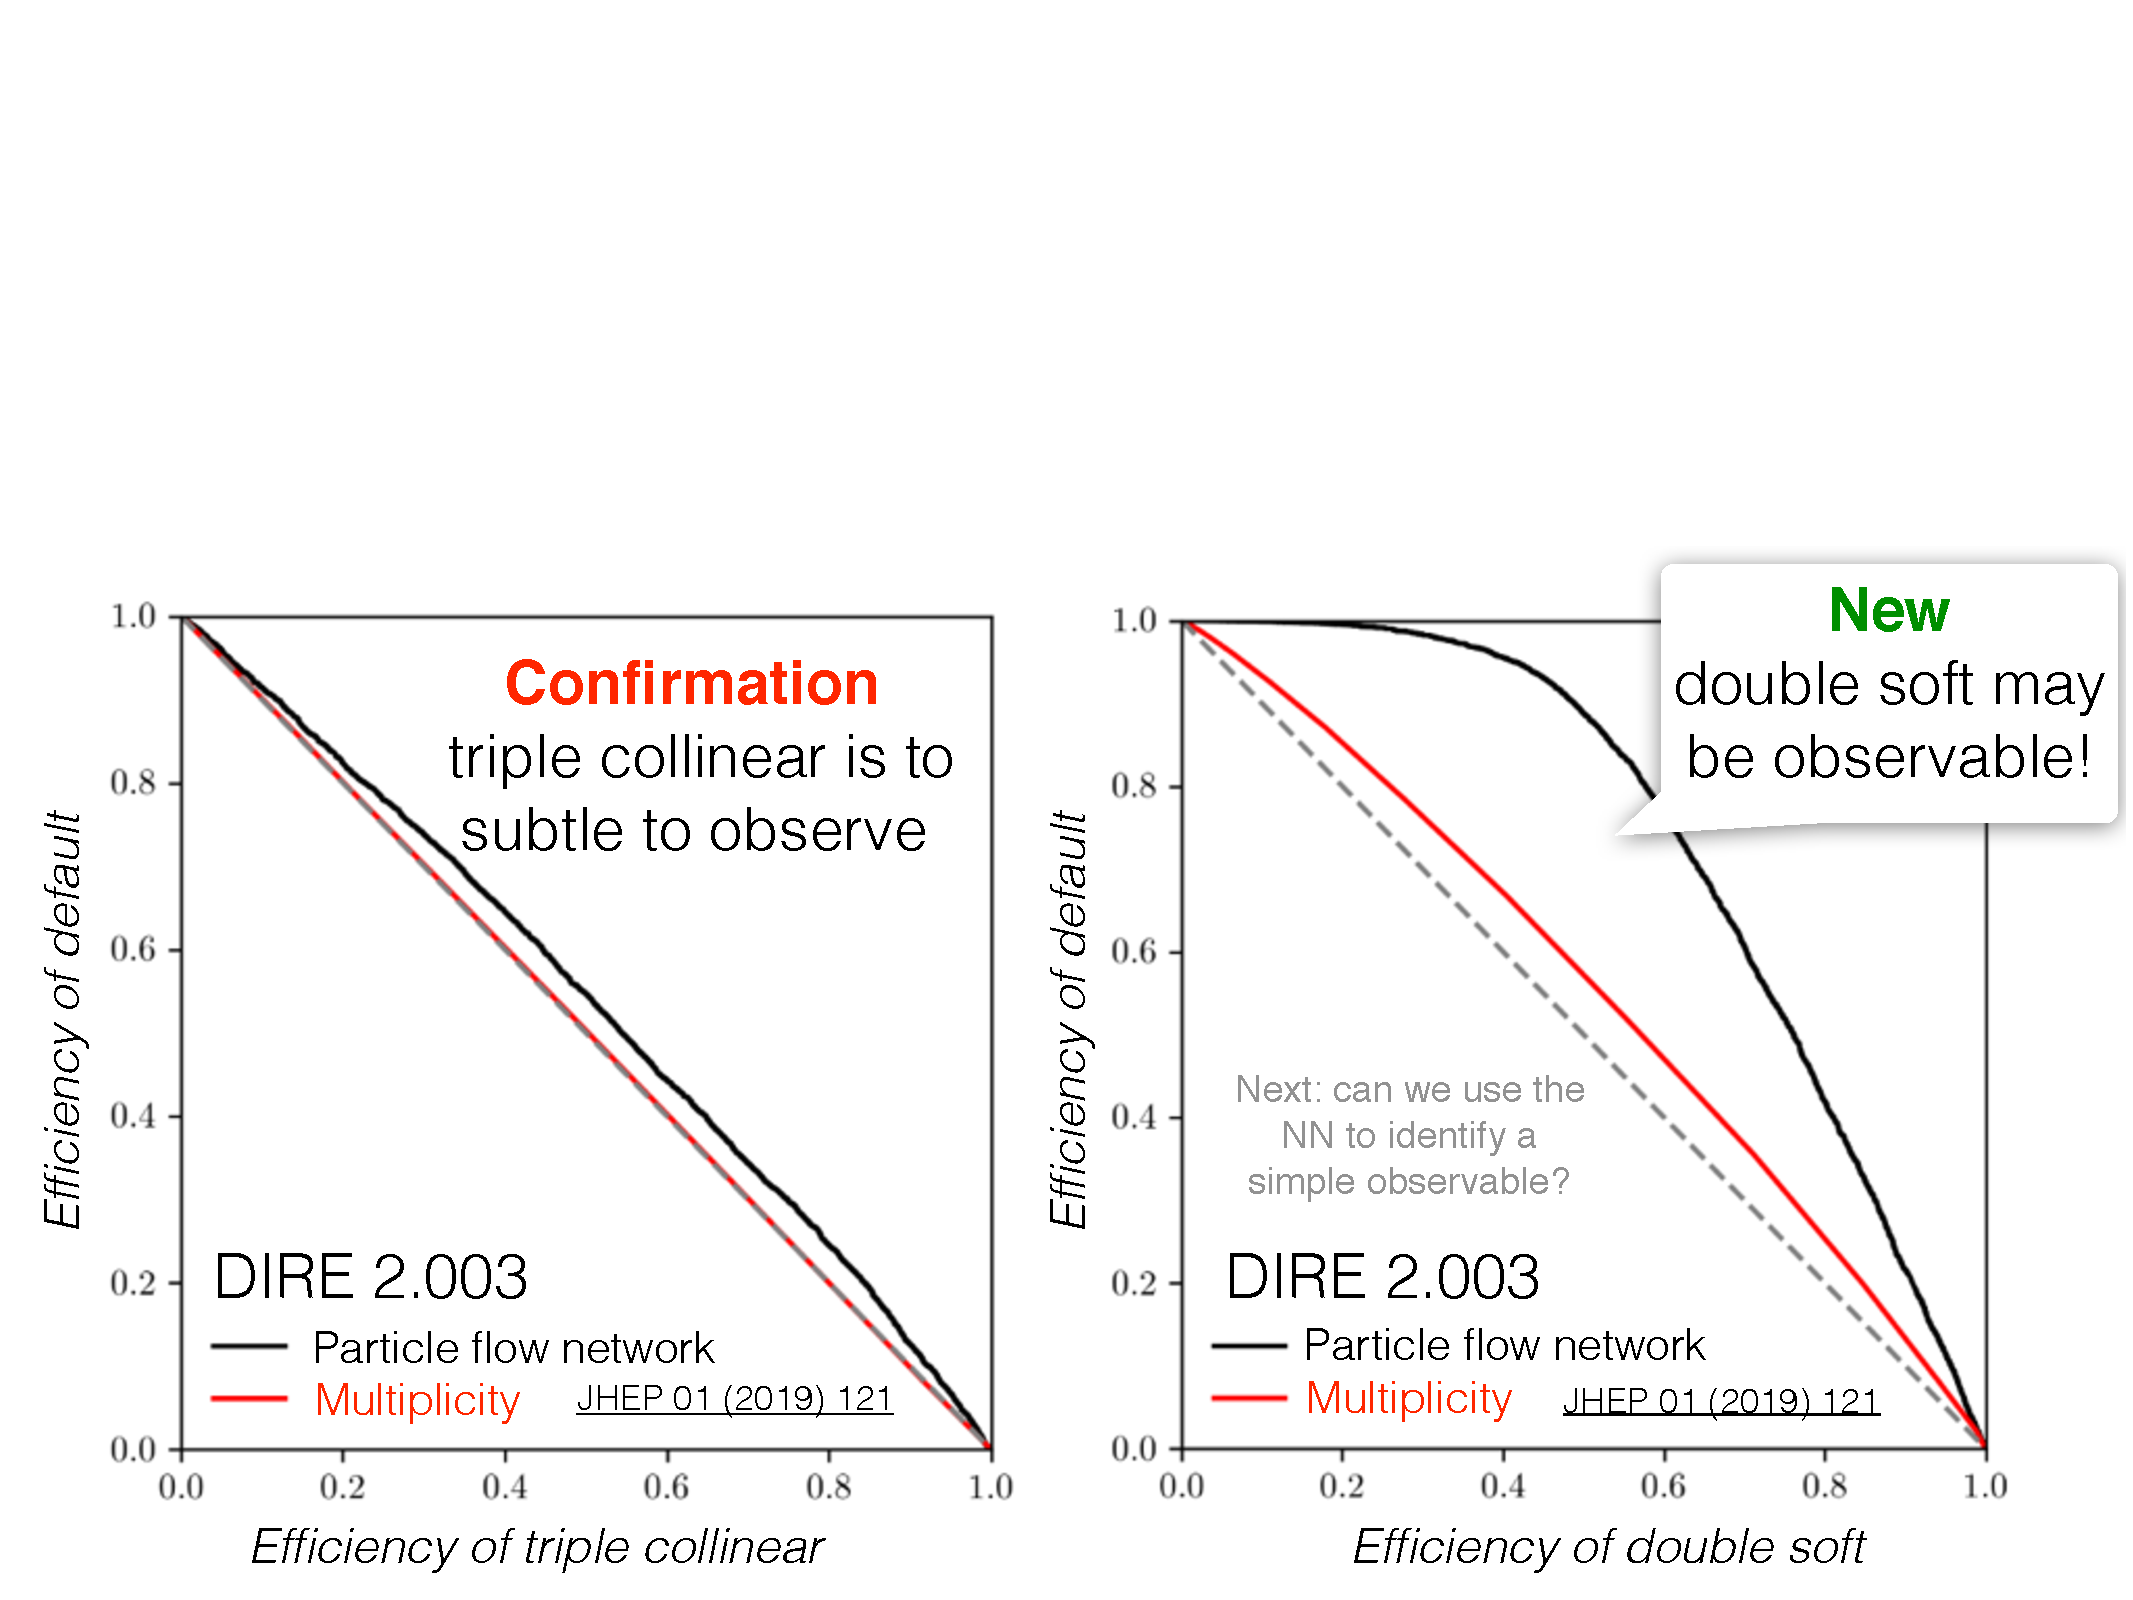
\includegraphics[width=0.85\textwidth]{figs/triplecollinear.pdf}
\caption{Receiver operating characteristic (ROC) curves for pseudo-data with and without the triple collinear splitting functions (left) and with and without the double soft splitting functions (right).  The performance of a classifier using just the jet constituent multiplicity is compared with a deep neural network acting on the full observable jet phase space.  For reference, a classifier that cannot distinguish between the two models is depicted with a dashed line.  Better classifiers are up and to the right.}
\label{fig:jets:np:triplecollinearNN}
\end{figure}




